\section{Ion implant}
We can use the following equation to calculate the carrier distribution after implantation:
\begin{equation}
N(x)
=
N_p \exp\left(-\frac{(x-R_p)^2}{2\Delta R_p^2}\right)
=
\frac{Q}{\sqrt{2\pi}\Delta R_p}\exp\left(-\frac{(x-R_p)^2}{2\Delta R_p^2}\right)
\end{equation}

Where the projected range ($R_p$) and the projected straggle ($\Delta R_p$) need to be looked up in tables \footnote{ISBN 3-8023-1588:Hoppe Bernhard, Mikroelektronik 2, Page 48, Table 3.2} or looked up using an online tool like the one linked in the footnote\footnote{\url{http://cleanroom.byu.edu/rangestraggle}}

\begin{figure}[H]
	\centering
	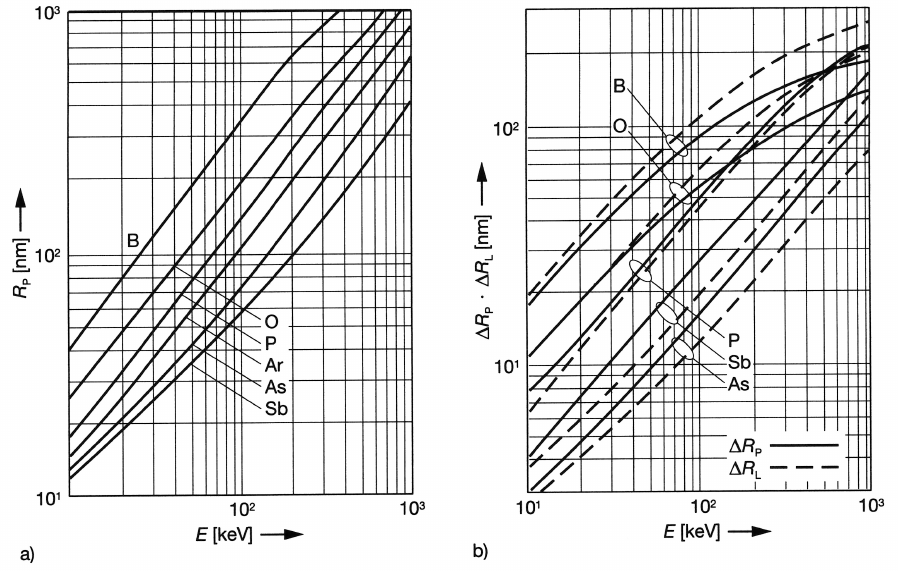
\includegraphics[width=0.75\textwidth]{ion_implant.png}
	\caption{$R_p$ and $\Delta R_p$ in silicon}
	\label{graphics_range_and_straggle}
\end{figure}

\begin{mdframed}[linewidth=2pt,linecolor=red]
If you do implant before the diffusion just set $x_v=R_p$
\end{mdframed}